\section{Study Design}
\label{sec:study-design}

\subsection{Benchmark Corpus}

We draw workloads from the HeCBench suite \cite{jinBenchmarkSuiteImproving2023}, focusing on CUDA and OpenMP target-offload programs because they are both common GPU programming models and represent distinct source/build ecosystems \cite{kadoshQuantifyingOpenMPStatistical2023}.
The final corpus contains 95 benchmark programs (56 CUDA, 39 OpenMP), which expose 254 first-invocation GPU kernels (155 CUDA, 99 OpenMP); we preserve the suite's natural CUDA/OpenMP mix rather than artificially balancing the two.
Profiling the corpus on four NVIDIA GPUs yields 1{,}016 samples, and each sample induces three precision-specific \rai labels (FP16/FP32/FP64), so the profiler-derived ground-truth space contains 3{,}048 precision-specific evaluation points before any model-query filtering.

\begin{table*}[t]
  \centering
  \caption{Profiled GPUs and DRAM-level balance points used for \bandwidthbound/\computebound classification.}
  \label{tab:gpu-specs}
  \small
  \setlength{\tabcolsep}{4pt}
  \begin{tabular}{lcccc}
    \toprule
    & RTX 3080 & A10 & A100 & H100 \\
    \midrule
    Base architecture & Ampere (GA102) & Ampere (GA102) & Ampere (GA100) & Hopper (GH100) \\
    Compute capability & 8.6 & 8.6 & 8.0 & 9.0 \\
    Memory bandwidth (GB/s) & 760 & 600 & 1{,}555 & 3{,}360 \\
    L2 cache (MB) & 5 & 6 & 40 & 50 \\
    FP16 peak (TFLOP/s) & 30.55 & 15.62 & 77.97 & 133.82 \\
    FP32 peak (TFLOP/s) & 30.55 & 15.62 & 19.49 & 66.91 \\
    FP64 peak (TFLOP/s) & 0.477 & 0.244 & 9.75 & 33.45 \\
    \midrule
    FP16 balance point (FLOP/byte) & 40.20 & 26.03 & 50.14 & 39.83 \\
    FP32 balance point (FLOP/byte) & 40.20 & 26.03 & 12.53 & 19.91 \\
    FP64 balance point (FLOP/byte) & 0.63 & 0.41 & 6.27 & 9.96 \\
    \bottomrule
  \end{tabular}
\end{table*}


We profile on four GPUs chosen to span different memory and compute regimes: RTX~3080, A10, A100, and H100.
\autoref{tab:gpu-specs} lists their characteristics and the resulting DRAM-level balance points used for \bandwidthbound/\computebound classification.
The architectural question is therefore not whether models generalize to all accelerators; it is whether the same prompting strategy remains useful across noticeably different NVIDIA deployment targets.

\begin{figure}[t]
  \centering
  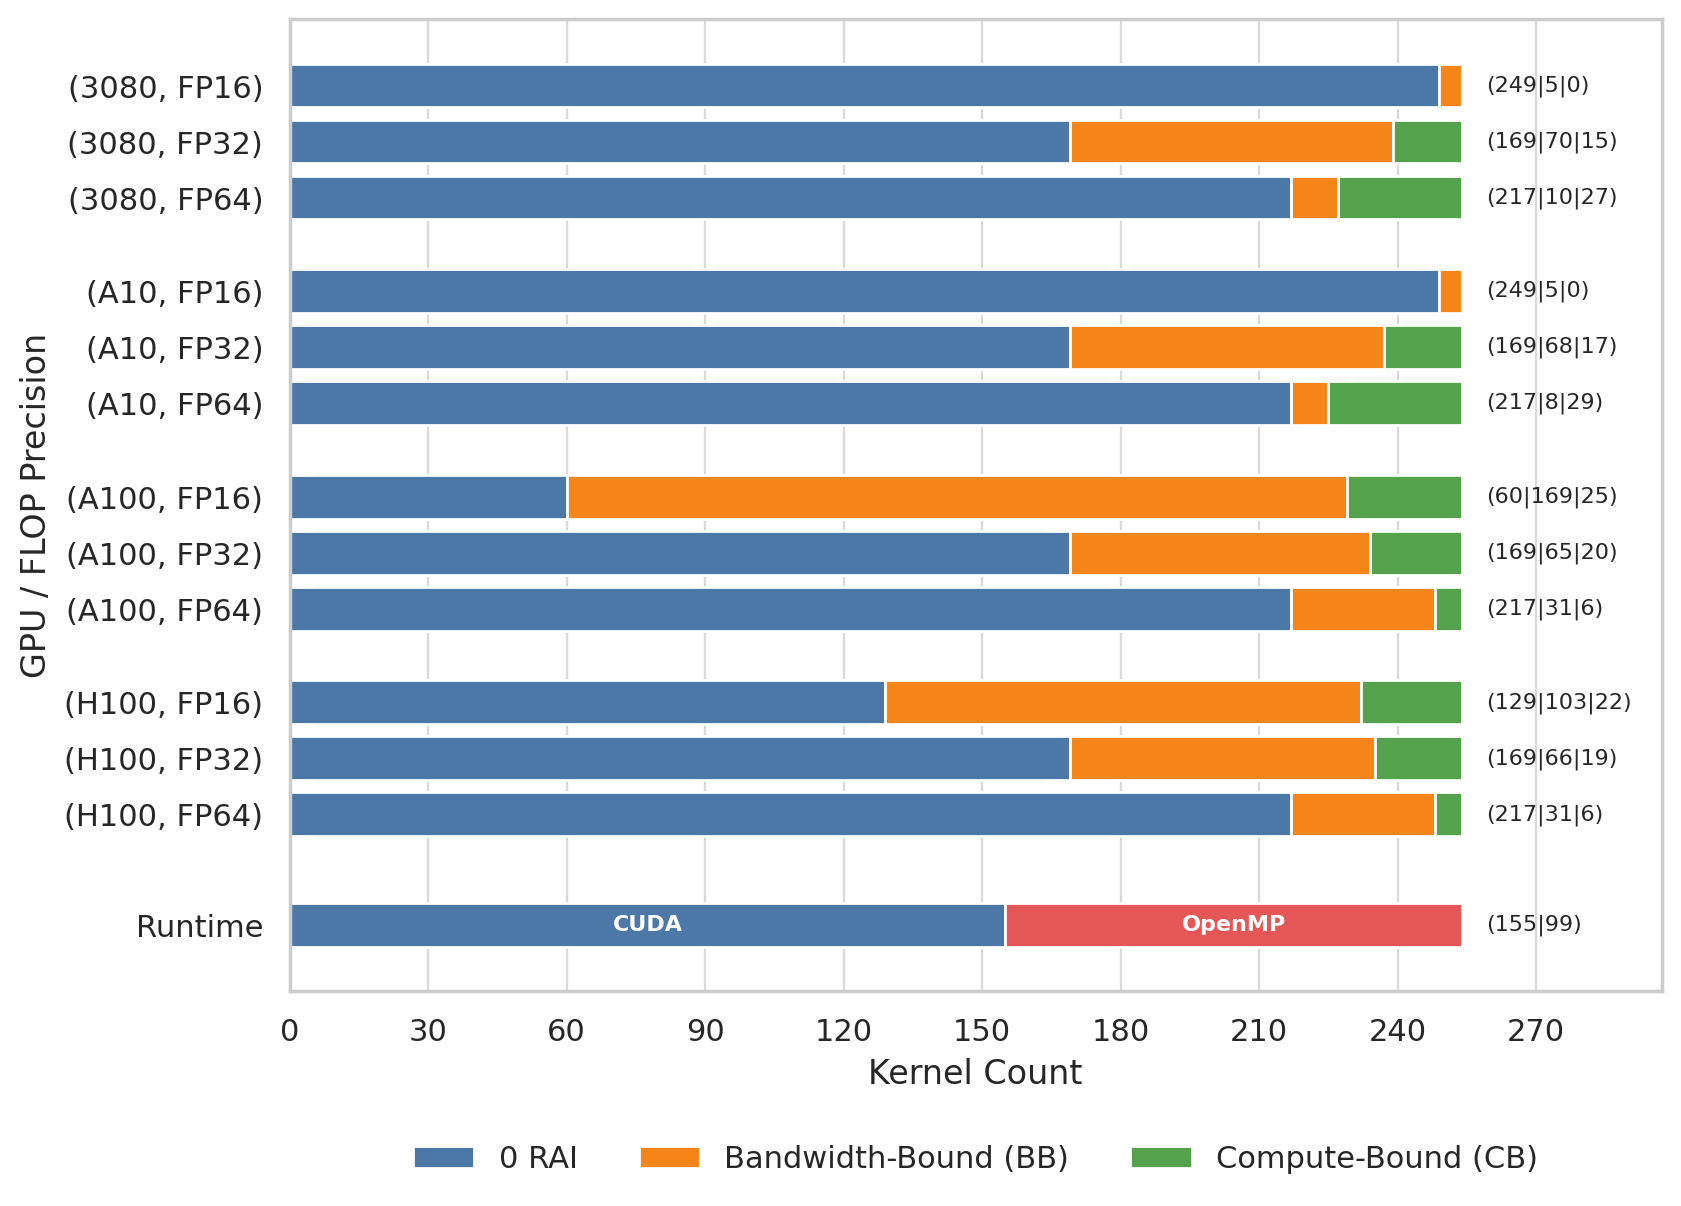
\includegraphics[width=\linewidth]{figures/gt_distribution_by_gpu_precision.png}
  \caption{Ground-truth \rai class distribution by GPU and precision.
  Zero-valued \rai cases dominate every precision, nonzero FP16 cases concentrate on A100/H100, and the nonzero \bandwidthbound/\computebound mix varies by device.
  These imbalances motivate separate evaluation of zero detection, nonzero regression, and nonzero \bandwidthbound/\computebound triage.}
  \Description{Stacked bars showing many zero-RAI cases in every precision, with nonzero FP16 concentrated on A100 and H100 and different bandwidth-bound versus compute-bound mixes by GPU.}
  \label{fig:gt-distribution}
\end{figure}

\autoref{fig:gt-distribution} highlights the resulting class imbalance.
Across the full 1{,}016 samples, FP16 has 687 zero cases, FP32 has 676, and FP64 has 868, and FP16 is especially architecture-sensitive because the A100/H100 binaries contain many more nonzero FP16 measurements than the 3080/A10.
This is precisely why we separate the evaluation tasks instead of reporting a single aggregate error number.

\subsection{Models and Sample Accounting}

\begin{table}[t]
  \centering
  \caption{The three off-the-shelf LLMs studied, sorted by release date.
  Costs are per million tokens (input\,/\,output) and context limits are maximum input\,/\,output tokens, as of March 2026.}
  \label{tab:llm-comparison}
  \scriptsize
  \setlength{\tabcolsep}{4pt}
  \begin{tabular}{llcc}
    \toprule
    Model & Released & \$/1M (in/out) & Max tok.\ (in/out) \\
    \midrule
    \texttt{GPT OSS 120B} & 2025-08-05 & 0.039 / 0.19 & 131K / 131K \\
    \opus & 2026-02-04 & 5.00 / 25.00 & 872K / 128K \\
    \gptfivefour & 2026-03-05 & 2.50 / 15.00 & 922K / 128K \\
    \bottomrule
  \end{tabular}
\end{table}


We study three off-the-shelf LLMs (\autoref{tab:llm-comparison}): the two frontier models \gptfivefour and \opus, and the roughly 100$\times$ cheaper open-source baseline \gptoss.
We do not fine-tune the models, train task-specific heads, or expose runtime feedback inside the prediction loop, and all comparisons use the two released prompt configurations that differ only by the presence of SASS (\sourceonly and \sourcesass).
The committed run script invokes one trial per sample for \texttt{openai/gpt-5.4}, \texttt{anthropic/claude-opus-4.6}, and \texttt{openai/gpt-oss-120b}, with the released client defaulting to temperature 0.2 and top-$p$ 0.1.

The frontier models were queried once per sample in the released evaluation subset, which is a limitation of the artifact, so we report coverage explicitly rather than hiding it inside aggregate metrics:
\begin{itemize}[leftmargin=1.2em]
  \item 3{,}048 \sourcesass and 3{,}048 \sourceonly predictions for \opus,
  \item 3{,}048 \sourcesass and 3{,}045 \sourceonly predictions for \gptfivefour, and
  \item 2{,}535 \sourcesass and 2{,}574 \sourceonly predictions for \gptoss.
\end{itemize}
\gptoss incompletions primarily reflect context-overflow or completion failures on long prompts.
For fair cross-model comparison we use the 732 samples completed by all three models in both prompt settings, and within-model source-versus-SASS comparisons are paired on the subset completed by both settings for that model.

\subsection{Evaluation Metrics}

We report a deliberately small set of metrics organized around the primary outcome (\bandwidthbound/\computebound regime classification) and a numeric diagnostic (\rai error).

\paragraph{Regime classification (primary).}
For nonzero cases we compare the predicted and expected side of the GPU-specific balance point: a kernel is \computebound when its \rai exceeds that balance point and \bandwidthbound otherwise.
Because the class ratios are uneven, we report balanced accuracy (macro recall), which cannot be inflated by predicting the majority class, and the released artifact additionally exports \computebound precision/recall/F1 so reviewers can see whether high recall comes from over-predicting the compute side.
If a model predicts zero for a truly nonzero kernel, we conservatively count it as a memory-side failure, since a zero prediction still fails to identify compute-side behavior.

\paragraph{Numeric \rai error (diagnostic).}
For nonzero cases we report the median absolute percent error of predicted \rai, where the percent error for precision $p$ is $100\,(\text{predicted}_p - \text{expected}_p)/\text{expected}_p$.
The distributions are heavy-tailed, so we emphasize medians and interquartile behavior rather than means.

\paragraph{Zero detection.}
Because the corpus is zero-heavy, we also report balanced accuracy on distinguishing zero from nonzero \rai; only an exact zero prediction counts as ``zero,'' and any positive or non-finite prediction is conservatively treated as ``nonzero.''
As reference points, always predicting zero yields 0.50 balanced accuracy on zero detection, and always predicting the majority nonzero class yields 0.50 on regime classification.

\subsection{Repeated-Query Consistency}

A single query per kernel cannot establish reliability, since LLM outputs are nondeterministic.
To characterize run-to-run variability without re-running the full grid, we select a small, deterministic, stratified panel of 24 kernels from the evaluated set using \texttt{select\_repeat\_trial\_kernels.py}.
The panel is chosen to span precision, proximity to the balance point, \bandwidthbound/\computebound class, runtime (CUDA/OpenMP), and a hard-versus-easy split based on the error-prone code features identified in our failure analysis (division, special math, reusable subexpressions, and loop-invariant floating-point work), rather than only low-error cases; selection is fully deterministic, with ties broken by name so the panel reproduces exactly.
We then resample the models on this panel, repeating each query four times across all four GPUs and both evidence settings (no kernel perturbation), and measure two kinds of consistency: the coefficient of variation of predicted \rai across repeats, and whether the \bandwidthbound/\computebound call is unanimous across repeats.

\subsection{Static Baselines (Deferred)}

To establish that the LLM signal is worth its cost beyond off-the-shelf prompting, we additionally plan a like-for-like comparison against lightweight static baselines defined for our exact target: a context-only median predictor, deterministic source-lexical and SASS-mnemonic heuristics, and lightweight learned static predictors over the same source- and disassembly-derived features.
Because we are still constructing these baselines to match the per-precision DRAM-level Roofline target, we defer the comparison to a subsequent revision (RQ4) and report it as future work rather than a measured result here.

\subsection{Exploratory Failure Analysis}

The released artifact also contains an auxiliary feature-voting pipeline that uses inexpensive LLMs to label source patterns such as division, special math, reusable subexpressions, and loop-invariant floating-point work.
We retain this analysis because it helps characterize where prediction errors cluster, but we treat it as exploratory: the feature labels are not human-validated, so we use them to describe repeated failure patterns rather than to make causal claims, and we summarize association strength with Cliff's $\delta$ in the appendix.
